
%%
%%  Beam Loading Paper '17
%% ***************************
%%  Veronica K. Berglyd Olsen
%%

\documentclass[aps,prstab,reprint,amsmath,amssymb,groupedaddress]{revtex4-1}
\bibliographystyle{apsrev4-1}

\usepackage{hyperref}
\hypersetup{colorlinks=true, citecolor=blue, urlcolor=blue, linkcolor=blue}

\usepackage{graphicx}


% Custom Commands
%*****************

% Text
%~ \newcommand{\eq}[1]{Eq. \ref{#1}}
%~ \newcommand{\fig}[1]{Fig. \ref{#1}}
%~ \newcommand{\tbl}[1]{Table \ref{#1}}

% Math
\newcommand{\unit}[1]{\,\mathrm{#1}}
\newcommand{\funit}[2]{\,\mathrm{#1}/\mathrm{#2}}
\newcommand{\mexp}[1]{\mathrm{e}^{#1}}
\newcommand{\nexp}[1]{\times 10^{#1}}

% ******************************************************************************************************************** %
\begin{document}
% ******************************************************************************************************************** %

%~ Eric's Comments
%~ Sec N: Beam loading [in this section we describe the interesting physics, based on a single parameters set]
%~ - describe proton beam wake structure [similar to that of a modulated proton beam] (simulation results to show:
%~   unloaded wake)
%~ - by varying the current of the electron beam, the electron beam may load the wake and the longitudinal field can be
%~   flatten and energy spread reduced [well known result, Tzoufras] 
%~ - the electron beam blows out the remaining plasma electrons. The transverse fields are dominated by the linear
%~   focusing fields originating from the ion background, leading to emittance preservation of the part of the electron
%~   beam inside the bubble [loading of a quasi-linear wake, and still get emittance preservation: this is new]
%~   (simulation results to show: loaded wake, with bubble - many different aspects of this, trans., long. field,
%~   electron densities etc. )
%~ - the acceleration and the transverse emittance stable on long timescales (simulation results to show: transverse and
%~   longitudinal phase spaces, space long simulation)
%~ - in this regime, emittance preservation is robustness to drive-witness offset [this is new] (simulation results to
%~   show: transverse and longitudinal phase spaces, long offset simulation)
%~ Sec N+1: Parameter optimization, or, parameter scaling [in this section we describe how to optimize the electron
%~ beam, and preferably some scalings]
%~ - how to select electron beam parameters:
%~ - longitudinal parameters bunch length and current (simulations results to show: overloaded/underloaded cases)
%~ - transverse parameters of electron emittance / matching [too large, outside bubble.  Do we see increased head
%~   erosion -> faster decay]?  (simulations results to show: evolution of high emittance vs low emittance cases)
%~ (- plasma density?)


%~ Patric's Comments
%~ - Self-modulation as a driver
%~ - SM does not reach blow out
%~ - SM does not preserve emittance and produces large energy spread and parameters may evolve along the accelerator,
%~   not desirable
%~ - Beam loading for narrow energy spread
%~ - Beam loading in linear regime (old papers from SLAC in the 80's, then Katsouleas for PWFA) and nonlinear regime
%~   (Tzoufras) well know
%~ - Propose "new regime" in the SM case, beam loading and blowout to get emittance preservation
%~ - Limitation as for PWFA driver, must use some of the W bunch to reach the blowout, it is kind of like the early SLAC
%~   experiments (84GeV) where the W-bunch is like the D-bunch in these experiments, but in a plasma prepared by the p+
%~   bunch and the SM
%~ - maybe also something about the fact that 200pC in a 60µm bunch corresponds to a 1kA current, much larger than the
%~   p+ bunch current, because of the fact that the wakefields are driven my multiple bunches?
%~ As for N+2, I am a firm supporter of on-axis injection ... and most of the issue with that has to do with the plasma
%~ ramp, otherwise it would be a non-issue (assuming of course that one can split the plasma in two sections). It is in
%~ itself a topic of research, so I think we can only state a few things ...


\title{Emittance preservation of an electron bunch in a loaded quasi-linear plasma wakefield}

\author{Veronica K. Berglyd Olsen}
\email[]{v.k.b.olsen@cern.ch}

\author{Erik Adli}
\affiliation{University of Oslo, Oslo, Norway}

\author{Patric Muggli}
\affiliation{Max Planck Institute for Physics, Munich, Germany}
\affiliation{CERN, Geneva, Switzerland}

\date{\today}

\begin{abstract}
We investigate beam loading and emittance preservation for a high-charge electron beam being accelerated in quasi-linear
plasma wakefield driven by a short proton beam. The structure of the wakefield is similar to that of a long, modulated
proton beam. By selecting transverse and longitudinal electron beam parameters in order to appropriately load the wake,
we show that the bulk of the electron beam can be accelerated without significant emittance growth.
\end{abstract}

\maketitle

\section[\label{S:I}]{Introduction}

% interested from SMI/AWAKE
% requirements for AWAKE Run 2

The preliminary design of AWAKE Run 2 proposes to use two plasma sections. The first section of 4m is the SMI stage. The
electron beam will be injected into the modulated proton beam before stage two, where acceleration will occur. As the
$e_z$ field will decrease due to the gap between the two cells, it is desireable to keep this as short as possible
\cite{adli:2016}.

\section[\label{S:M}]{Method}
%- explain analogy of short-bunch, SMI case, by referring to earlier Veronica-papers
%- simulation setup PIC/quickpic OS

The main focus of this study has been on the beam loading of the electron beam. In order to eliminate other factors that
may affect this, we have tried several approaches to create a stable drive beam structure based on previous SMI studies
[citations].

Our first approach was to use a premodulated, short proton beam with the same structure as a section of the full AWAKE
proton drive beam. These studies were done using the full PIC code Osiris \cite{fonseca:2002} using 2D
cylindrical-symetric simulations. The proton beam was pre-modulated by a clipped cosine function to the longitudinal
density profile, with a period matching the wavelength, $\lambda_p$, of the plasma. The length was limited to
$26\cdot\lambda_p$, and the electron beam injected after the 20th micro-bunch \cite{berglyd_olsen:2015}. We performed
several parameter scans with this setup, testing for optimal charge as well as beam length
\cite{adli:2016, berglyd_olsen:2016}.

[Add something about the optimal results]

In order to evaluate the quality of the beam, we also needed to study its emittance. Full PIC codes like Osiris are
vulnerable to numerical growth of emittance caused by the ``numerical Cherenkov effect'' \cite{godfrey:1974}. This is a
know issue with the Yee EMF solver, which causes the phase velocity of electromagnetic fields to be lowet than $c$,
while the beam moves very close to $c$. The effect can be mitigated somewhat by a the Lehe solver \cite{lehe:2013}, but
the effect is still prominent in the the high density regions of the electron beam.

In order to study the emittance evolution of the beam we used QuickPIC, a fully relativistic 3D PIC code
\cite{huang:2006, an:2013}.

\subsection[\label{S:M:Setup}]{Drive Beam Parameters}

In these simulations we use a single proton drive bunch that sets up a wakefield comparable to that which we expect to
see from the self-modulated SPS beam in AWAKE. The baseline AWAKE drive beam contains $3\nexp{11}$ protons
\cite{gschwendtner:2016}. Only half of these are driving the wakefield, presuming the self-modulation is seeded in the
middle of the unmodulated bunch. In addition. a significant portion of the protons are lost during self-modulation. The
needed gap between the two plasma cells also contributes to a decreased density of protons near the axis, and some of
the field is drained by other protons seeing an accelerating face within the drive beam. In total, the expected peak
$E_{z}$ field of $~2\funit{GV}{m}$ in the first plasma cell drops to $500-600\funit{MV}{m}$ in the second cell
\cite{awake_collaboration:2016}. A single proton beam of $1.46\nexp{10}$, or $2.34\unit{nC}$ and $7\unit{kA}$, is needed
to drive an $E_{z}$ field of a comparable magnitude.

The single bunch approach was chosen to reduce simulation time for the 3D simulations, and to create a stable
environment for the witness beam. We are not considering the evolution of the proton beam in this test setup, so to
prevent the proton beam from evolving radially, we increased its mass.

The basline AWAKE drive beam current is insufficient to produce a plasma bubble. The plasma electrons are depleted to
around $65\%$ of nominal plasma density at the injection point of the electron beam. This condition is replicated in out
single bunch case. The single bunch setup also uses the baseline proton energy $W_{pb} = 400\unit{GeV}$.

\subsection[\label{S:M:Setup}]{Witness Beam Parameters}

The witness beam in our simulation differs from AWAKE baseline parameters on several key points. Initial beam energy is
set such that $\gamma_{eb} = \gamma_{pb} = 426.3$. This is to eliminate the problem of initial de-phasing of the witness
beam. AWAKE baseline witness beam energy for Run 1 is $W_{eb} = 10-20\unit{MeV}$ \cite{gschwendtner:2016}. Beam loading
of a short witness beam is sensitive to initial position. AWAKE Run 2 will likely require a higher initial energy, but a
$W_{eb} = 30--50\unit{MeV}$ is sufficient to minimise de-phasing \cite{berglyd_olsen:2015}. For this case we have
eliminated it entirely in order to reduce the number of variables in our parameter scans.

Earlier simulations with witness beam $\sigma_{r} = 100\unit{\mu m}$ causes the beam radius to rapidly shrink as the
beam enters the plasma \cite{berglyd_olsen:2016}. This is due to a mismatch between beam emittance and the plasma
density. The relation is given by
\begin{align}
    \beta = \frac{\sigma_r^2}{\epsilon_g} = \frac{\lambda_p}{2\pi}\sqrt{2\gamma_{rel}}, \label{EQ:Matched}
\end{align}
where $\lambda_{p}$ is the plasma wavelength. In these simulations we have used matched beams for emittances between
$2$ and $6\unit{\mu m}$.

\section[\label{S:BL}]{Beam Loading}

%~ Eric's Comments
%~ Sec N: Beam loading [in this section we describe the interesting physics, based on a single parameters set]

%~ - describe proton beam wake structure [similar to that of a modulated proton beam] (simulation results to show:
%~   unloaded wake)

The structure of the single drive beam setup behaves similarly to the self-modulated case. However, since the drive
beam is prevented from significant evolution in this simulation setup, we are presented with an idealised case where
the electron witness beam sees consistent fields.

\begin{figure}
    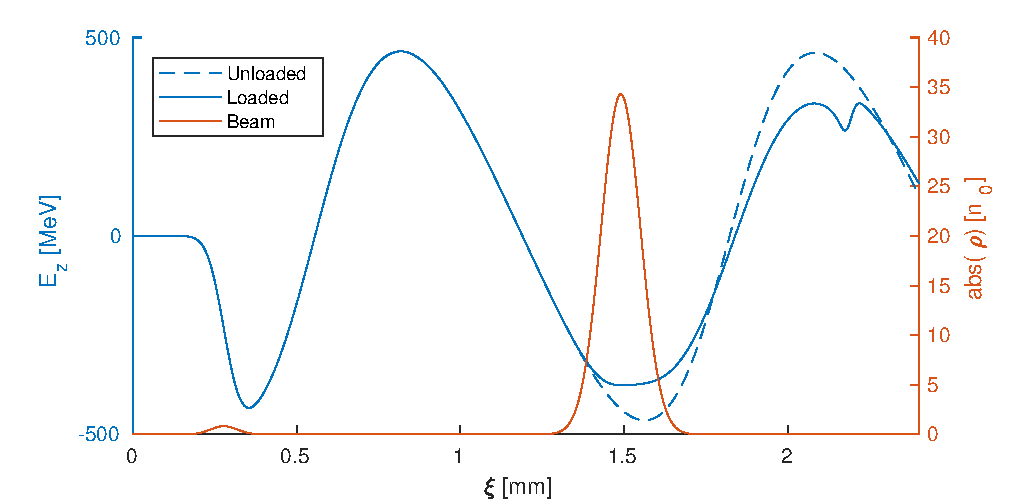
\includegraphics[width=0.99\linewidth,trim={4mm 0mm 4mm 0mm},clip]{figures/beamLoading}
    \label{Fig:BeamLoading}
    \caption{Comparison between the unloaded longitudinal e-field (no witness beam) and the loaded e-field along the
        axis. The magnitude of the beam density along the axis is shown for reference. The beams travel towards the
        left. $\xi = z - tc$ is the position in the simulation box. The beam density is in units of plasma density
        $n_{0} = 7\nexp{-14}\unit{cm}^{-3}$.}
\end{figure}



%~ - by varying the current of the electron beam, the electron beam may load the wake and the longitudinal field can be
%~   flatten and energy spread reduced [well known result, Tzoufras]

\begin{figure}
    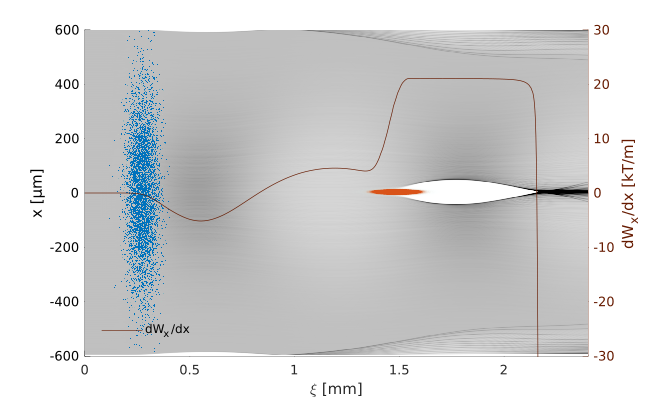
\includegraphics[width=0.99\linewidth,trim={4mm 0mm 4mm 0mm},clip]{figures/plasmaDenTWake}
    \label{Fig:PlasmaDenTWake}
    \caption{}
\end{figure}



%~ - the electron beam blows out the remaining plasma electrons. The transverse fields are dominated by the linear
%~   focusing fields originating from the ion background, leading to emittance preservation of the part of the electron
%~   beam inside the bubble [loading of a quasi-linear wake, and still get emittance preservation: this is new]
%~   (simulation results to show: loaded wake, with bubble - many different aspects of this, trans., long. field,
%~   electron densities etc. )



%~ - the acceleration and the transverse emittance stable on long timescales (simulation results to show: transverse and
%~   longitudinal phase spaces, space long simulation)



%~ - in this regime, emittance preservation is robustness to drive-witness offset [this is new] (simulation results to
%~   show: transverse and longitudinal phase spaces, long offset simulation)

\section[\label{S:PO}]{Parameter Optimisation}

%~ Sec N+1: Parameter optimization, or, parameter scaling [in this section we describe how to optimize the electron
%~ beam, and preferably some scalings]
%~ - how to select electron beam parameters:
%~ - longitudinal parameters bunch length and current (simulations results to show: overloaded/underloaded cases)
%~ - transverse parameters of electron emittance / matching [too large, outside bubble.  Do we see increased head
%~   erosion -> faster decay]?  (simulations results to show: evolution of high emittance vs low emittance cases)
%~ (- plasma density?)


\section[\label{S:D}]{Discussion}
\section[\label{S:C}]{Conclusion}

% discussion of optimal electron beam parameters
% implications for AWAKE Run 2

\bibliography{Bibliography}

% ******************************************************************************************************************** %
\end{document}
% ******************************************************************************************************************** %
